\documentclass[aspectratio=149]{beamer}
\usepackage[english]{babel}
\usepackage[utf8x]{inputenc}
\usepackage{amsmath, amsthm}
\usepackage{amssymb}
\usepackage{tikz}
\usetikzlibrary{calc,shapes,positioning, arrows.meta}
\usepackage{graphicx, subfig}
%\usepackage[ruled,linesnumbered]{algorithm2e}

%\renewcommand{\bibsection}{}
%\newcommand{\tikzmark}[1]{\tikz[overlay,remember picture] \node (#1) {};}

%%algorithm
%\let\oldnl\nl% Store \nl in \oldnl
%\newcommand{\nonl}{\renewcommand{\nl}{\let\nl\oldnl}}% Remove line number for one line
%% new colour
%\definecolor{darkcerulean}{rgb}{0.03, 0.27, 0.49}
%% underbrace with normal font
%\newcommand{\bunderbrace}[2]{%
%  \begin{array}[t]{@{}c@{}}
%  \underbrace{#1}\\ 
%    #2
%  \end{array}
%}

\makeatletter
\let\save@measuring@true\measuring@true
\def\measuring@true{%
  \save@measuring@true
  \def\beamer@sortzero##1{\beamer@ifnextcharospec{\beamer@sortzeroread{##1}}{}}%
  \def\beamer@sortzeroread##1<##2>{}%
  \def\beamer@finalnospec{}%
}
\makeatother

%%% maths
\newcommand{\HH}{\ensuremath{\mathbb{H}}}
\newcommand{\X}{\ensuremath{\mathbb{X}}}
\newcommand{\Y}{\ensuremath{\mathbb{Y}}}
\newcommand{\measurable}{\ensuremath{\mathcal{B}_b}}
\DeclareMathOperator{\Exp}{\mathbb{E}}
\DeclareMathOperator{\pr}{\mathbb{P}}
\DeclareMathOperator{\KL}{KL}
\DeclareMathOperator{\mise}{MISE}
\DeclareMathOperator{\mse}{MSE}
\DeclareMathOperator{\N}{\mathcal{N}}
\DeclareMathOperator{\ent}{ent}
\newcommand{\lp}{\ensuremath{\mathbb{L}_p}}
\def\real{\mathbb{R}}
\newcommand{\norm}[2]{\ensuremath{\Vert #1 \Vert_{#2}}}
\newcommand{\supnorm}[1]{\norm{#1}{\infty}}
\newcommand{\variation}[1]{\ensuremath{\frac{\delta F}{\delta #1}}}


%%% arrows
\newcommand{\tikzmark}[1]{\tikz[overlay,remember picture] \node (#1) {};}


\usetikzlibrary{shapes.arrows}
\tikzset{
        myarrow/.style={
        draw,
        fill=blue,
        single arrow,
        minimum height=5.5ex,
        single arrow head extend=1ex
           }
}
\newcommand{\arrowright}{%
\tikz [baseline=-0.5ex]{\node [myarrow,rotate=0] {};}
}


% set the paths for all the graphic objects
\graphicspath{{Images/}}

\mode<presentation>
{
  \usetheme[compress]{Singapore}
  \usecolortheme{default} % or try albatross, beaver, crane, ...
  \usefonttheme{default}  % or try serif, structurebold, ...
  \setbeamertemplate{navigation symbols}{}
  \setbeamertemplate{footline}[ ]
  \setbeamertemplate{caption}[numbered]
} 

%%% TITLE
\title{Solving Fredholm Integral Equations through Wasserstein Gradient Flows}
\author{Francesca R. Crucinio\\
\small{with Adam M. Johansen \& Arnaud Doucet}}
\date{25 June 2020}

\begin{document}

%~~~INTRO~~~

\begin{frame}
  \titlepage
\end{frame}

%\begin{frame}{Outline}
%\tableofcontents
%\end{frame}

%\section{Motivation}
%\begin{frame}{Motivation}
%
%{\large \textbf{\textcolor{darkcerulean}{Why Fredholm integral equations of the first kind?}}}
%\begin{itemize}
%\item Model the task of reconstructing a signal $f$ from an observed distorted signal $h$ when the type of distortion $g$ is known.
%\item Have applications in e.g. indirect density estimation, image processing, inverse boundary problems for PDE.
%\item Ill-posed.
%\end{itemize}
%\vskip 10pt
%{\large \textbf{\textcolor{darkcerulean}{Why SMC?}}}
%\begin{itemize}
%\item In real-world applications the analytic form of $h$ is often unknown, but observations from $h$ are available.
%\item Leads to stochastic rather than deterministic approximations of the signal $f$.
%\end{itemize}
%
%\end{frame}

%\begin{frame}{Objective}
%\begin{itemize}
%\item Provide stochastic approximations of the signal $f$ through SMC when the analytic form of $h$ is not known.
%\item Obtain theoretical guarantees for the SMC scheme and the corresponding estimator of the solution.
%\end{itemize}
%\end{frame}

\begin{frame}{Fredholm Integral Equations of the First Kind (FIE)}
\begin{equation*}
      \mu\tikzmark{a}(dy) = \int_{\X} K(x \tikzmark{b}\mid y)\rho\tikzmark{c}(dx)\ \qquad
\end{equation*}\\[2ex]
\centering

\tikz[remember picture]{\node(d){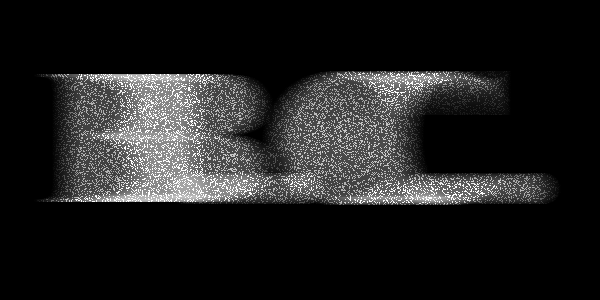
\includegraphics[width=0.43\textwidth]{BCnoisy}};}\qquad 
\tikz[remember picture]{\node(e){
\includegraphics[width=0.43\textwidth]{BC}};}
\qquad
\vskip 10pt
\tikz[remember picture]{\node(f){constant speed horizontal motion};}
  
  \tikz[remember picture,overlay]{
    \draw[->] (a.south) to (d.north) ;
    \draw[->] (c.south) to (e.north) ;
    \draw[->] (b.south) to (f.north) ;
    }
\end{frame}

\begin{frame}{Fredholm Integral Equations of the First Kind (FIE)}

\begin{itemize}
\item Applications: PDEs, indirect density estimation, signal reconstruction, causal inference, ...
\item Inverse ill posed problems
\item Solution methods often require discretisation/strong assumptions on $f$
\end{itemize}
\end{frame}

\begin{frame}{FIE - Solution method}
\begin{equation*}
\mu(dy) = \int_{\X} \rho(dx) K(y\mid x)\qquad \forall y \in \Y,
\end{equation*}
Take $\rho,\mu$ probability measures and $K$ a Markov transition density
\begin{equation*}
\rho^\star:= \text{argmin}\KL(\mu,\rho K)-\alpha\ent(\rho)
\end{equation*}
for some $\alpha>0$.
\pause

How?
\begin{align*}
\text{minimisation}\longrightarrow \text{PDE}\longrightarrow \text{SDE}
\end{align*}
\end{frame}

\begin{frame}{Gradient Flows}
\centering
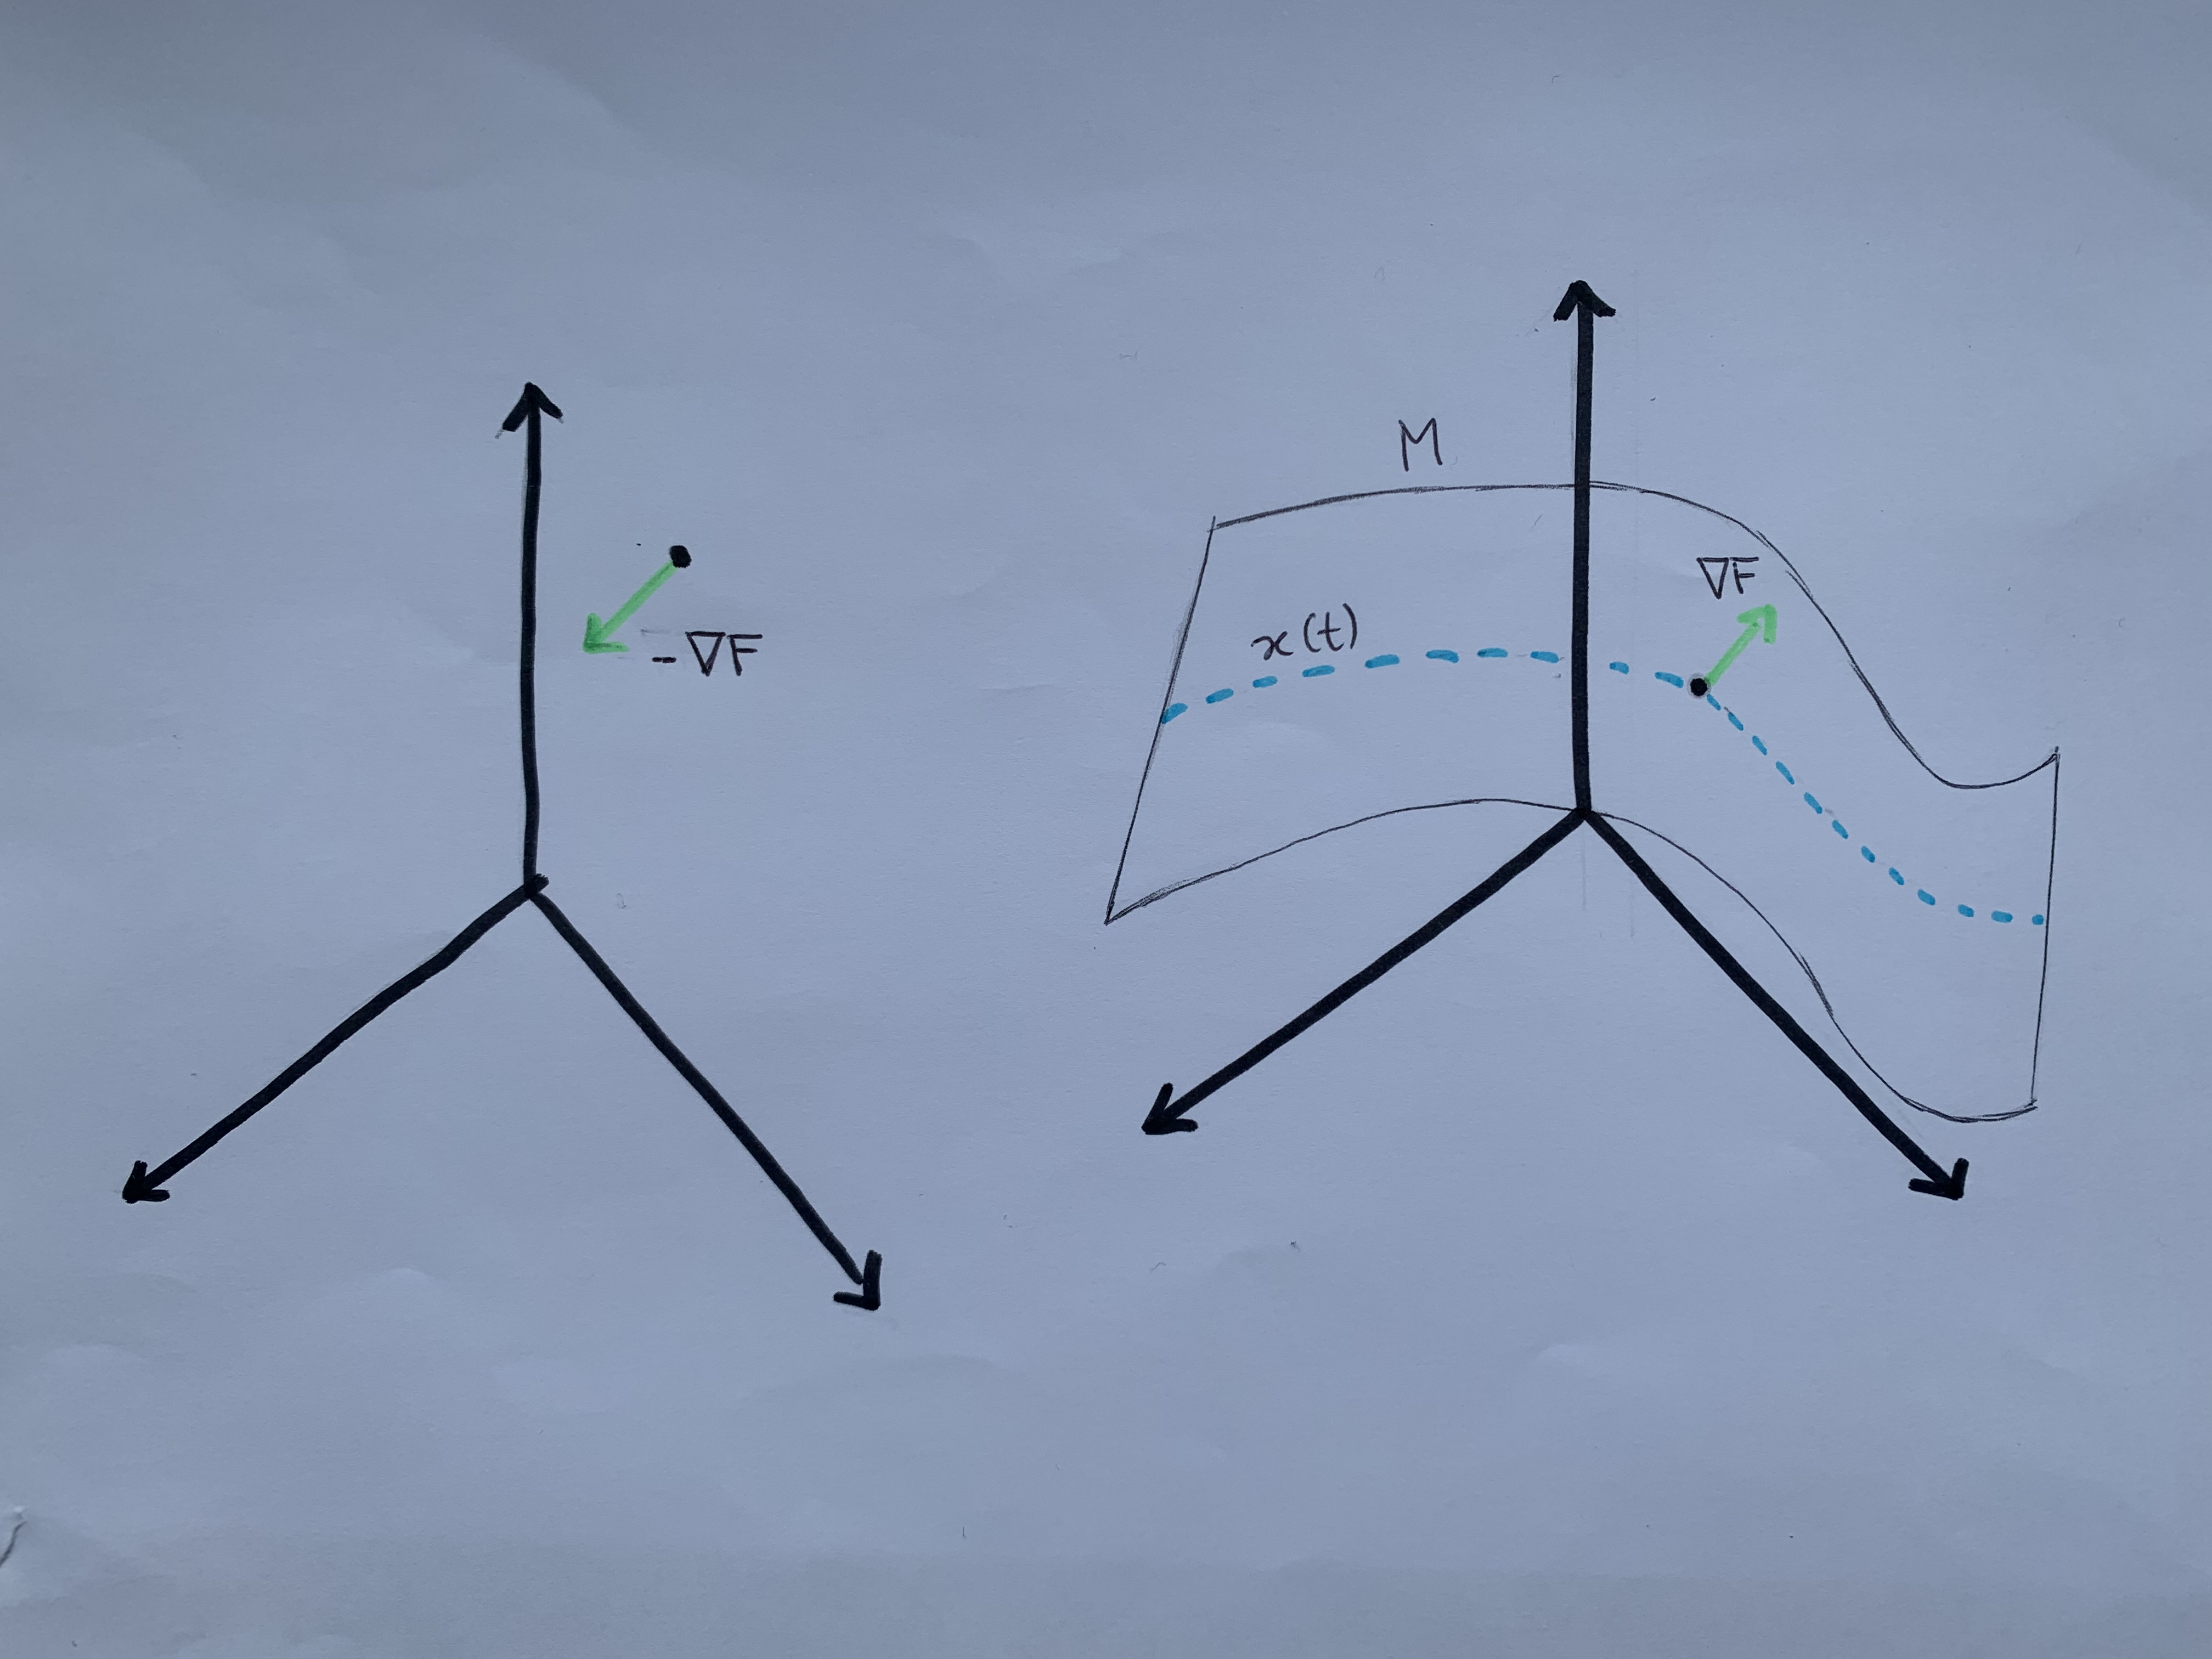
\includegraphics[width=0.7\textwidth]{gf}
\begin{align*}
x^\prime(t)=-\nabla F(x(t))
\end{align*}
\end{frame}

\begin{frame}{Wasserstein Gradient Flows (I)}
Take the manifold
\begin{align*}
\mathcal{P}_{2}^{ac}(\real^{d})=\left\lbrace \mu\in\mathcal{P}(\real^{d}):\int\norm{x}{2}^{2}\ d\mu(x)<\infty, \mu<<\mathcal{L}\right\rbrace 
\end{align*}
with distance
\begin{align*}
W_{2}(\mu,\nu):=\left(\inf_{\pi\in\Pi(\mu,\nu)}\int\norm{x-y}{2}^{2}\ d\pi(x,y)\right)^{1/2}
\end{align*}
\end{frame}


\begin{frame}{Wasserstein Gradient Flows (II)}
Curves in $\left(\mathcal{P}_{2}^{ac}(\real^{d}), W_2\right)$ are geodetics
\begin{align*}
\mu_s=((1-s)Id+st_{\mu}^{\nu})_{\#}\mu
\end{align*}
where $t_{\mu}^{\nu}$ is the unique transport map between $\mu$ and $\nu$ and $T_{\#}\mu$ denotes the push-forward measure
\begin{align*}
T_{\#}\mu(A)=\mu(T^{-1}(A)).
\end{align*}
\end{frame}

\begin{frame}{Wasserstein Gradient Flows (III)}

For $F:M\subset \real^d\mapsto \real$ the gradient flow equation is
\begin{align*}
x^\prime(t)=-\nabla F(x(t)).
\end{align*}

For $F:\mathcal{P}_{2}^{ac}(\real^{d})\mapsto \real$
we have\footnote{Jordan, Kinderlehrer, Otto (1998)}
\begin{align}
\label{eq:pde}
\partial_{t}\rho_{t}=-\nabla\cdot\left(\rho_{t}\variation{\rho_t}\right)
\end{align}
with $\variation{\rho_t}:=\frac{d}{d\epsilon}F(\rho+\epsilon\chi)_{|\epsilon=0}$.
\end{frame}

\begin{frame}{When is \eqref{eq:pde} well-behaved?}
We need:
\begin{itemize}
\item $F$ continuous, $F(\rho)<+\infty$ for some $\rho$
\item $F$ $\lambda-$convex: exists $\lambda\geq0$ s.t.
\begin{align*}
F\left(((1-s)Id+st_{\mu}^{\nu})_{\#}\mu\right)\leq(1-s)F(\mu)+sF(\nu)-\frac{\lambda}{2}s(1-s)W_{2}^{2}(\nu,\mu)
\end{align*}
\item $F$ is coercive: exists $r>0$ s.t.
\begin{align*}
\inf\left\lbrace F(\rho): \rho\in\mathcal{P}_{2}^{ac}(\real^{d}), \ \int\norm{x}{2}^{2}\ d\rho(x)\leq r\right\rbrace>-\infty
\end{align*}
\end{itemize}
\end{frame}

\begin{frame}{Then...}
The gradient flow PDE \eqref{eq:pde} has a unique solution for a given initial condition $\rho_0$.

\vspace{5mm}

For two initial conditions $\rho_0^1, \rho_0^2$ we have the estimate
\begin{align*}
W_{2}(\rho_{t}^{1},\rho_{t}^{2})\leq e^{-\lambda t}W_{2}(\rho_{0}^{1},\rho_{0}^{2}).
\end{align*}
\end{frame}

\begin{frame}{Gradient Flow for FIE - Assumptions}
\begin{equation*}
\mu(dy) = \int_{\X} \rho(dx) K(y\mid x)\qquad \forall y \in \Y, 
\end{equation*}


\begin{enumerate}
    \item $\X, \Y$ subsets of some Euclidean spaces with Borel $\sigma$-algebras; 
    \item $\mu, \rho$ densities with finite second moment;
    \item $K$ bounded and bounded away from 0, Lipschitz continuous with Lipschitz continuous gradient and $\lambda$-concave in $x$:
\begin{equation*}
x\mapsto K(x,y)+\frac{\lambda}{2}\norm{x}{2}^{2}
\end{equation*}
is concave for some $\lambda>0$ for all $y\in\Y$.
\end{enumerate}
\end{frame}

\begin{frame}{Gradient Flow for FIE}
\begin{equation*}
F(\rho) := \KL(\mu,\rho K)-\alpha\ent(\rho)
\end{equation*}
is continuous, coercive and $\lambda$ geodesically convex with $\lambda=0$ and has first variation
\begin{equation*}
\variation{\rho}\left(x\right)=-\int\mu\left(dy\right)\frac{K(x,y)}{\rho K(y)}+\alpha\left(1+\log\rho\left(x\right)\right).
\end{equation*}

\vspace{5mm}

\arrowright the gradient flow exist and is unique for each initial condition $\rho_0$
\end{frame}

\begin{frame}{Gradient Flow for FIE - PDE}
\begin{align*}
\partial_{t}\rho_{t}&=\nabla\cdot\left(\rho_{t}\nabla\variation{\rho_{t}}\right)\\
&=\nabla\cdot\left(\rho_t\left[-\int\mu\left(dy\right)\frac{\nabla K(x,y)}{\rho K(y)}+\alpha\nabla\log\rho\left(x\right)\right]\right)\\
&=-\nabla\cdot\left(\rho_{t}\int\mu\left(dy\right)\frac{\nabla K(x,y)}{\rho_{t}K(y)}\right)+\alpha\triangle\rho_{t}
\end{align*}
is a Fokker-Plank equation with corresponding SDE...
\end{frame}

\begin{frame}{Gradient Flow for FIE - SDE}
\begin{align*}
dX_{t}=\int\mu\left(dy\right)\frac{\nabla K(X_{t},y)}{\rho_{t}K(y)}dt+\sqrt{2\alpha}dW_{t},\quad X_{0}\sim\rho_{0}
\end{align*}

\begin{itemize}
\item McKean-Vlasov SDE
\item a strong solution exists and is unique
\item requires discretisation in time and space
\end{itemize}
\end{frame}

\begin{frame}{SDE - Implementation}
\begin{itemize}
\item discretisation in space: take $N$ copies of the SDE and use the resulting empirical measure instead of $\rho_t$
\begin{align*}
dX_{t}^{i,N}=\int\mu\left(dy\right)\frac{\nabla K(X_{t}^{i,N},y)}{\rho_{t}^{N}K(y)}dt+\sqrt{2\alpha}dW_{t}^{i},\quad\rho_{t}^{N}=\frac{1}{N}\sum_{i=1}^{N}\delta_{X_{t}^{i,N}}
\end{align*}
\item discretisation in time: Euler scheme
\begin{align*}
X_{n+1}^{i,N}& =X_{n}^{i,N}+\int\mu\left(dy\right)\frac{\nabla K(X_{n}^{i,N},y)}{\rho_{n}^{N}K(y)}\Delta t+\sqrt{2\alpha}\Delta W^{i},\\
&\rho_{n}^{N}=\frac{1}{N}\sum_{i=1}^{N}\delta_{X_{n}^{i,N}}
\end{align*}
\end{itemize}
\end{frame}

\begin{frame}{Toy Example}

\end{frame}

\begin{frame}{A second Toy Example}

\end{frame}
\begin{frame}{PET}

\end{frame}
\end{document}